%---------------------------------------------------------------------------%
%->> Section 4.4: 平台界面
%---------------------------------------------------------------------------%

\section{平台界面}

为支持离线知识构建与在线故障诊断两类任务，平台提供了与方法运行直接相关的三类主要界面，分别用于展示在线诊断过程、组织案例级任务以及查看故障指纹知识。这些界面共同构成了平台面向用户的主要交互入口，使任务执行状态、知识组织结果与中间诊断信息能够在统一环境中得到展示与管理。

\subsection{诊断执行界面}

诊断执行界面对应第 3.4 节所述的在线故障诊断过程。如图\ref{fig:user_sop_navigation}所示，界面左侧展示诊断消息、工具调用摘要和阶段性判断，右侧展示当前 SOP 节点图及其当前位置。借助这一界面，用户可以在同一视图中同时查看系统当前执行的动作、形成判断所依据的证据，以及当前所处的分支路径。

\begin{figure}[htbp]
    \centering
    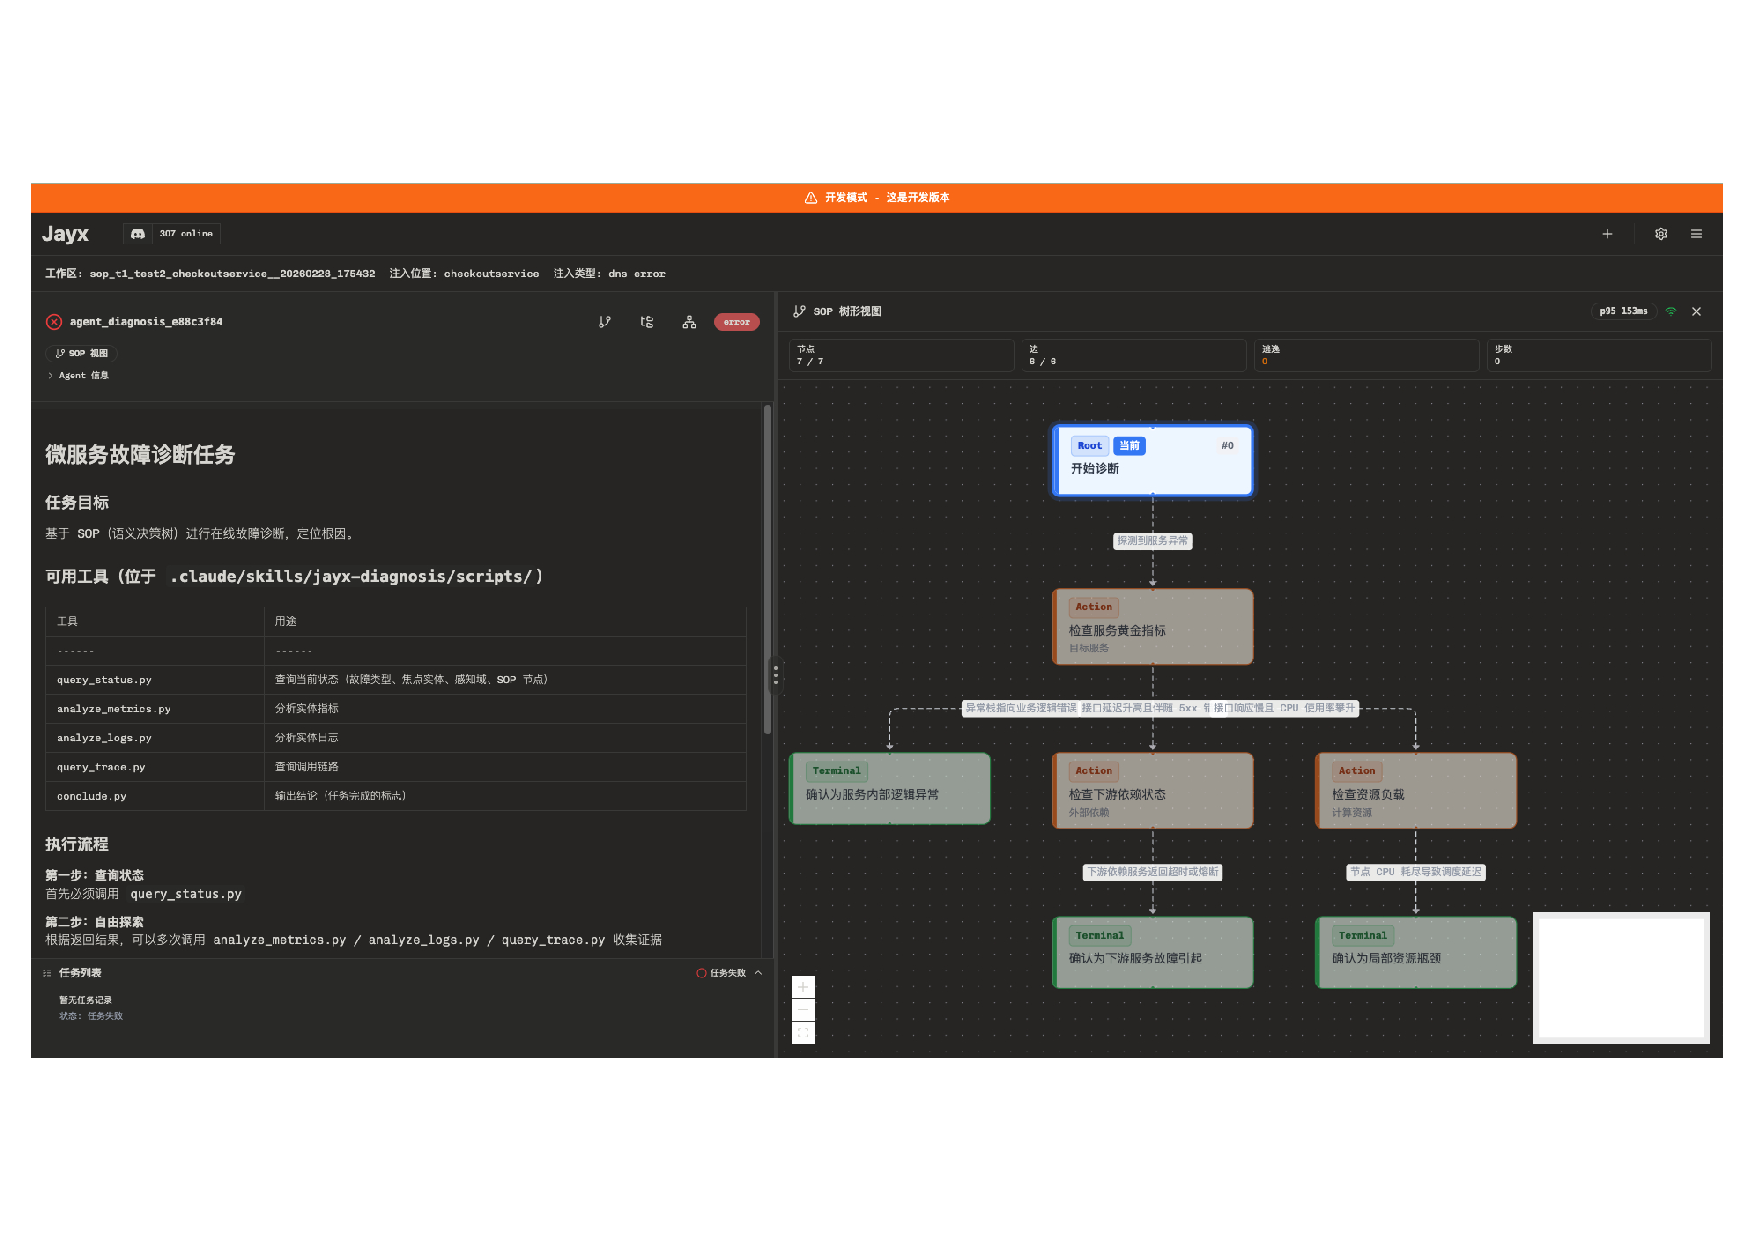
\includegraphics[width=0.96\textwidth]{Figures-Src/Chap4-System/user-interaction/fig1-sop-navigation.pdf}
    \bicaption{\enspace 诊断执行界面：左侧为 Agent 诊断日志与任务进度，右侧为 SOP 节点图}{\enspace Diagnosis Execution Interface: Left shows Agent diagnosis log and task progress, right shows SOP node graph}
    \label{fig:user_sop_navigation}
\end{figure}
\FloatBarrier

该界面用于将在线诊断过程与 SOP 路径状态对应起来。左侧消息区记录任务推进过程、工具返回结果和阶段性结论，右侧节点图同步标示当前节点及已执行路径。通过这一界面，用户不仅能够观察系统是否沿既有 SOP 持续推进，还能够识别其是否已经暂时脱离当前 SOP 并进入探索分支，从而更直观地理解诊断过程的演化状态。

\clearpage

\subsection{工作区界面}

工作区界面是案例级任务的统一入口，同时承载第 3.3 节对应的离线知识构建任务和在线诊断任务。如图\ref{fig:user_workspace}所示，每个工作区绑定一个具体案例。页面顶部展示工作区名称、注入位置和注入类型，中部以任务卡片形式展示该案例下的各类任务，并按照任务状态和任务类型进行分类。

\begin{figure}[htbp]
    \centering
    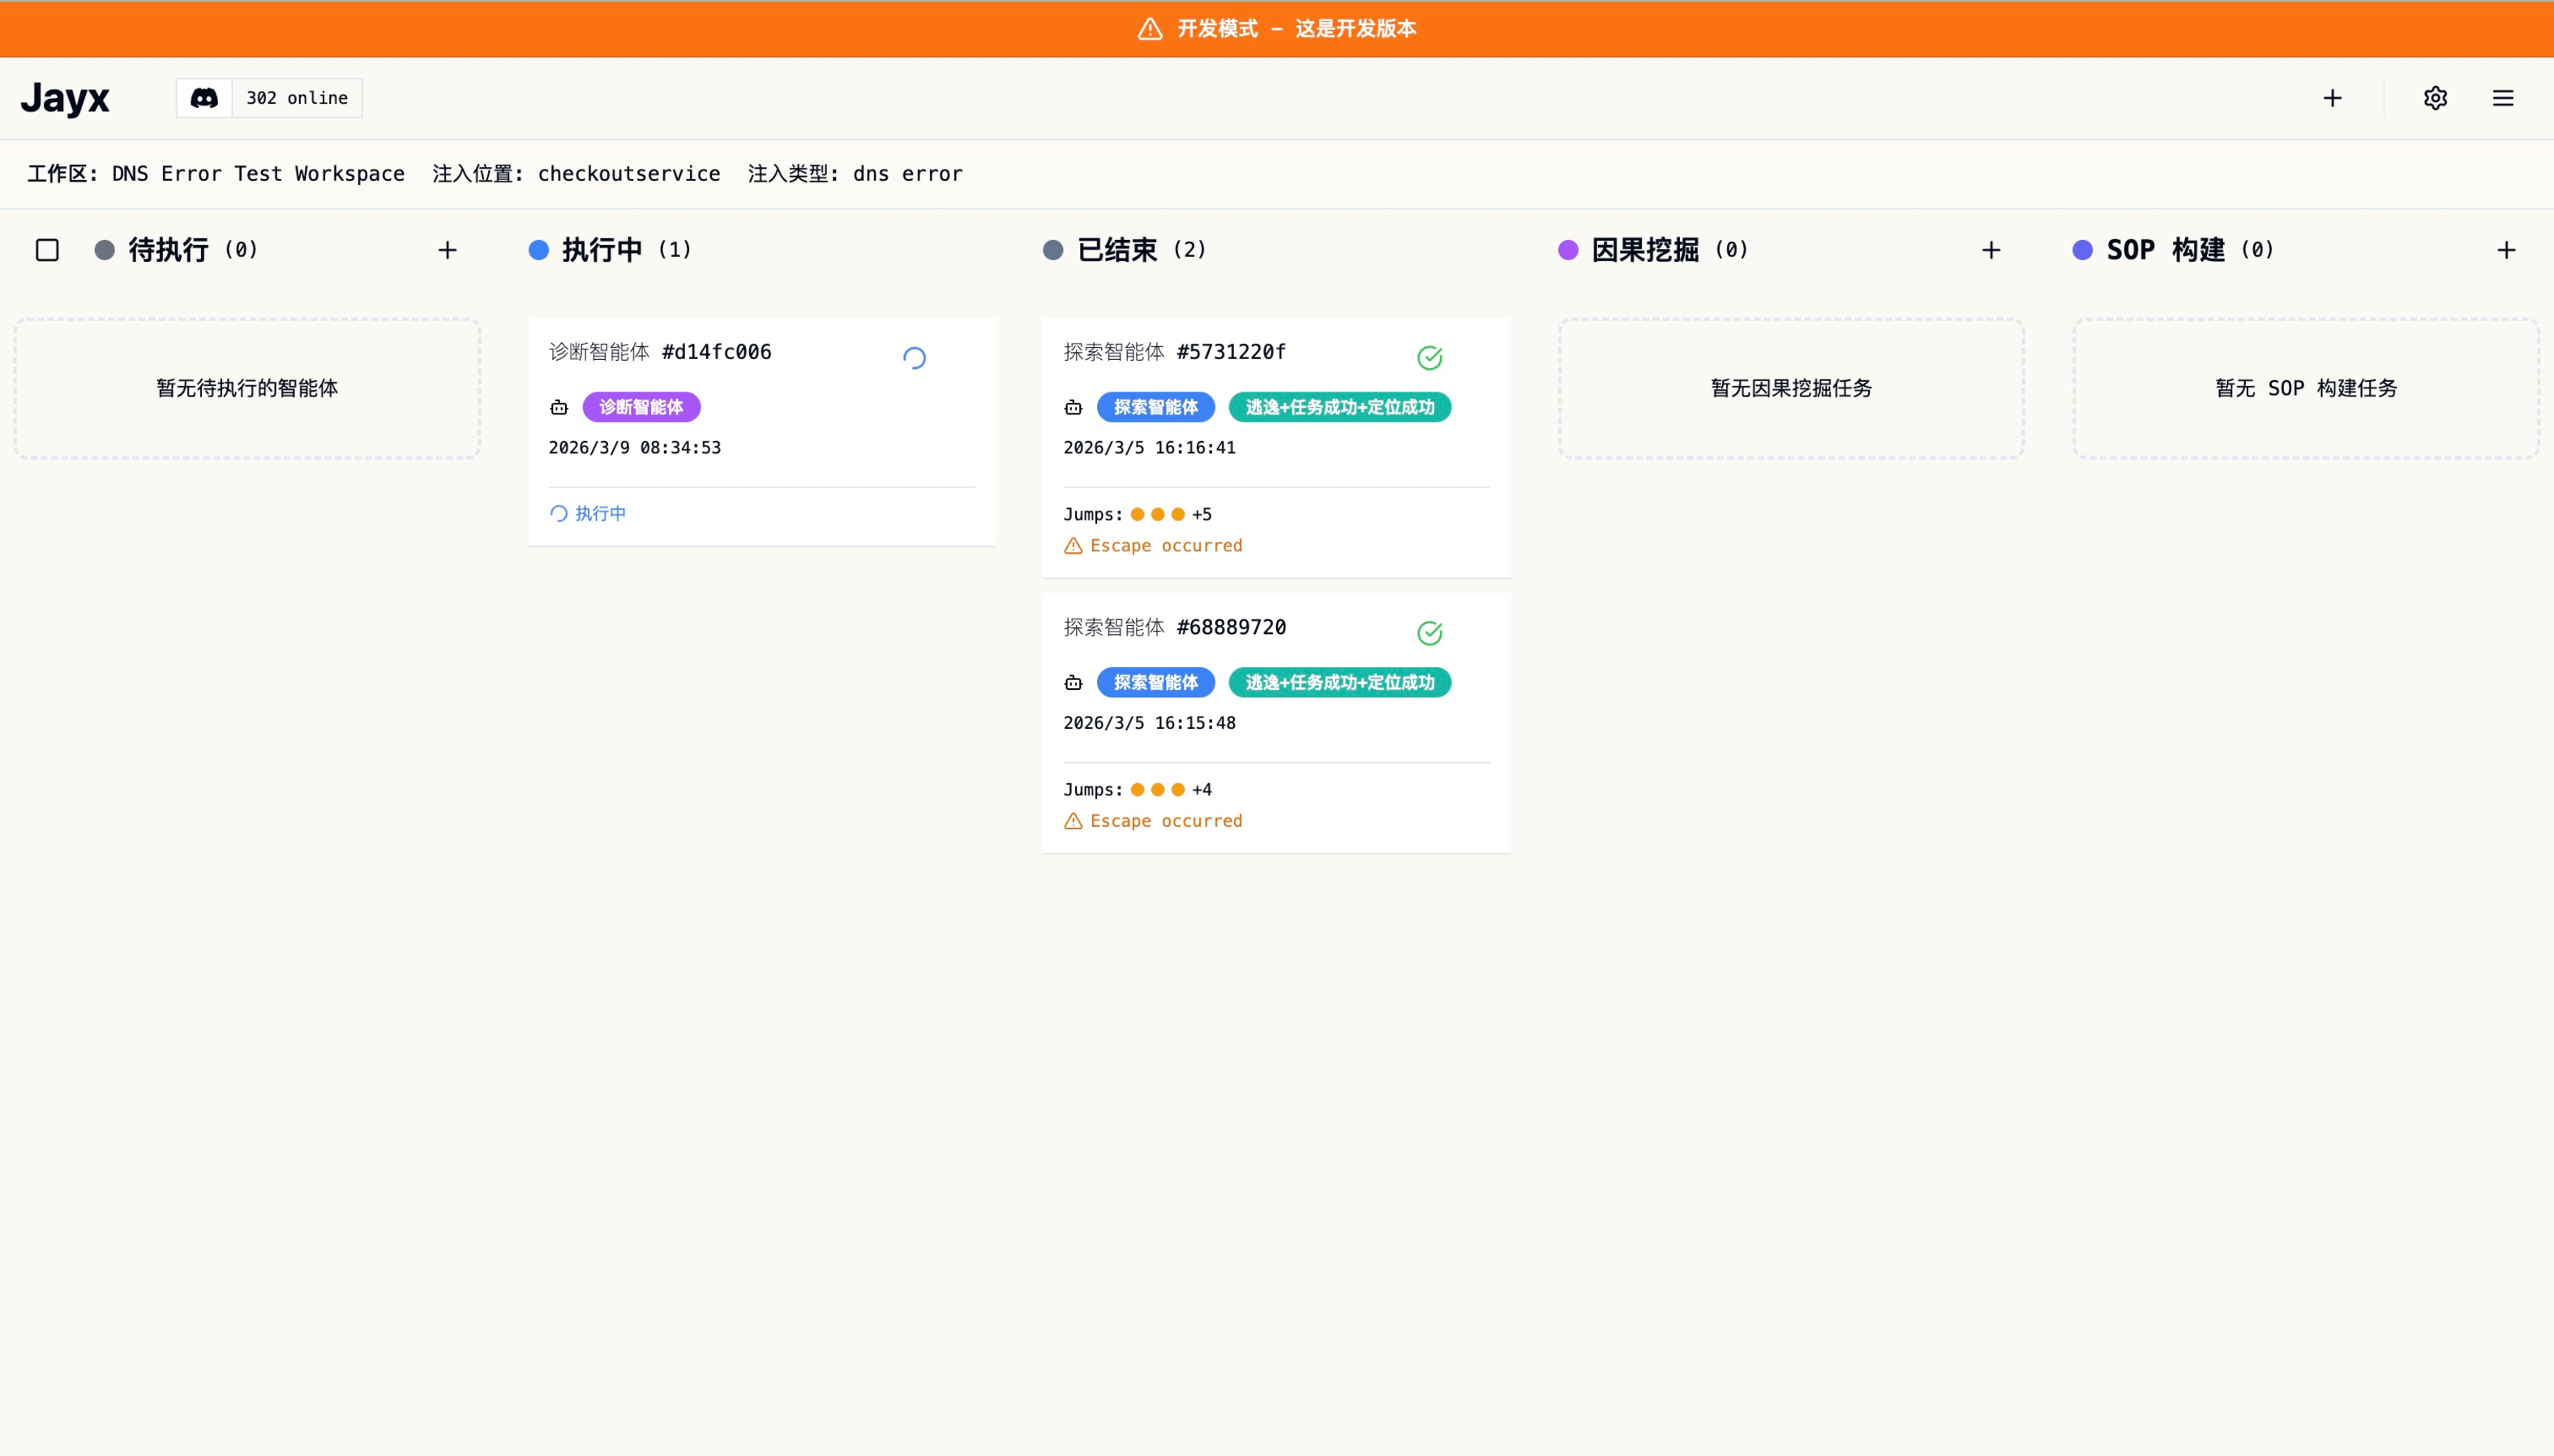
\includegraphics[width=0.96\textwidth]{Figures-Src/Chap4-System/user-interaction/fig2-workspace.pdf}
    \bicaption{\enspace 工作区中的案例信息与任务看板}{\enspace Case Context and Task Board in the Workspace}
    \label{fig:user_workspace}
\end{figure}
\FloatBarrier

工作区界面将同一案例相关的任务与中间结果组织在统一上下文下。在该界面中，用户可以创建诊断任务、探索任务、挖掘任务和 SOP 构建任务，也可以查看各任务对应的执行状态与输出结果。诊断结论、SOP 执行轨迹、决策单元提取结果以及 SOP 更新结果均保存在同一工作区内，便于围绕单个案例持续跟踪、回溯和管理。

\clearpage

\subsection{故障指纹界面}

故障指纹界面用于展示故障指纹库中的聚类结果及其样本分布。如图\ref{fig:user_fingerprint_3d}所示，系统采用 t-分布随机邻域嵌入（t-distributed Stochastic Neighbor Embedding，t-SNE）方法，将高维故障指纹投影到三维空间。界面左侧列表展示各聚类的编号、样本数和代表标签，右侧散点图展示样本在三维嵌入空间中的分布。

\begin{figure}[htbp]
    \centering
    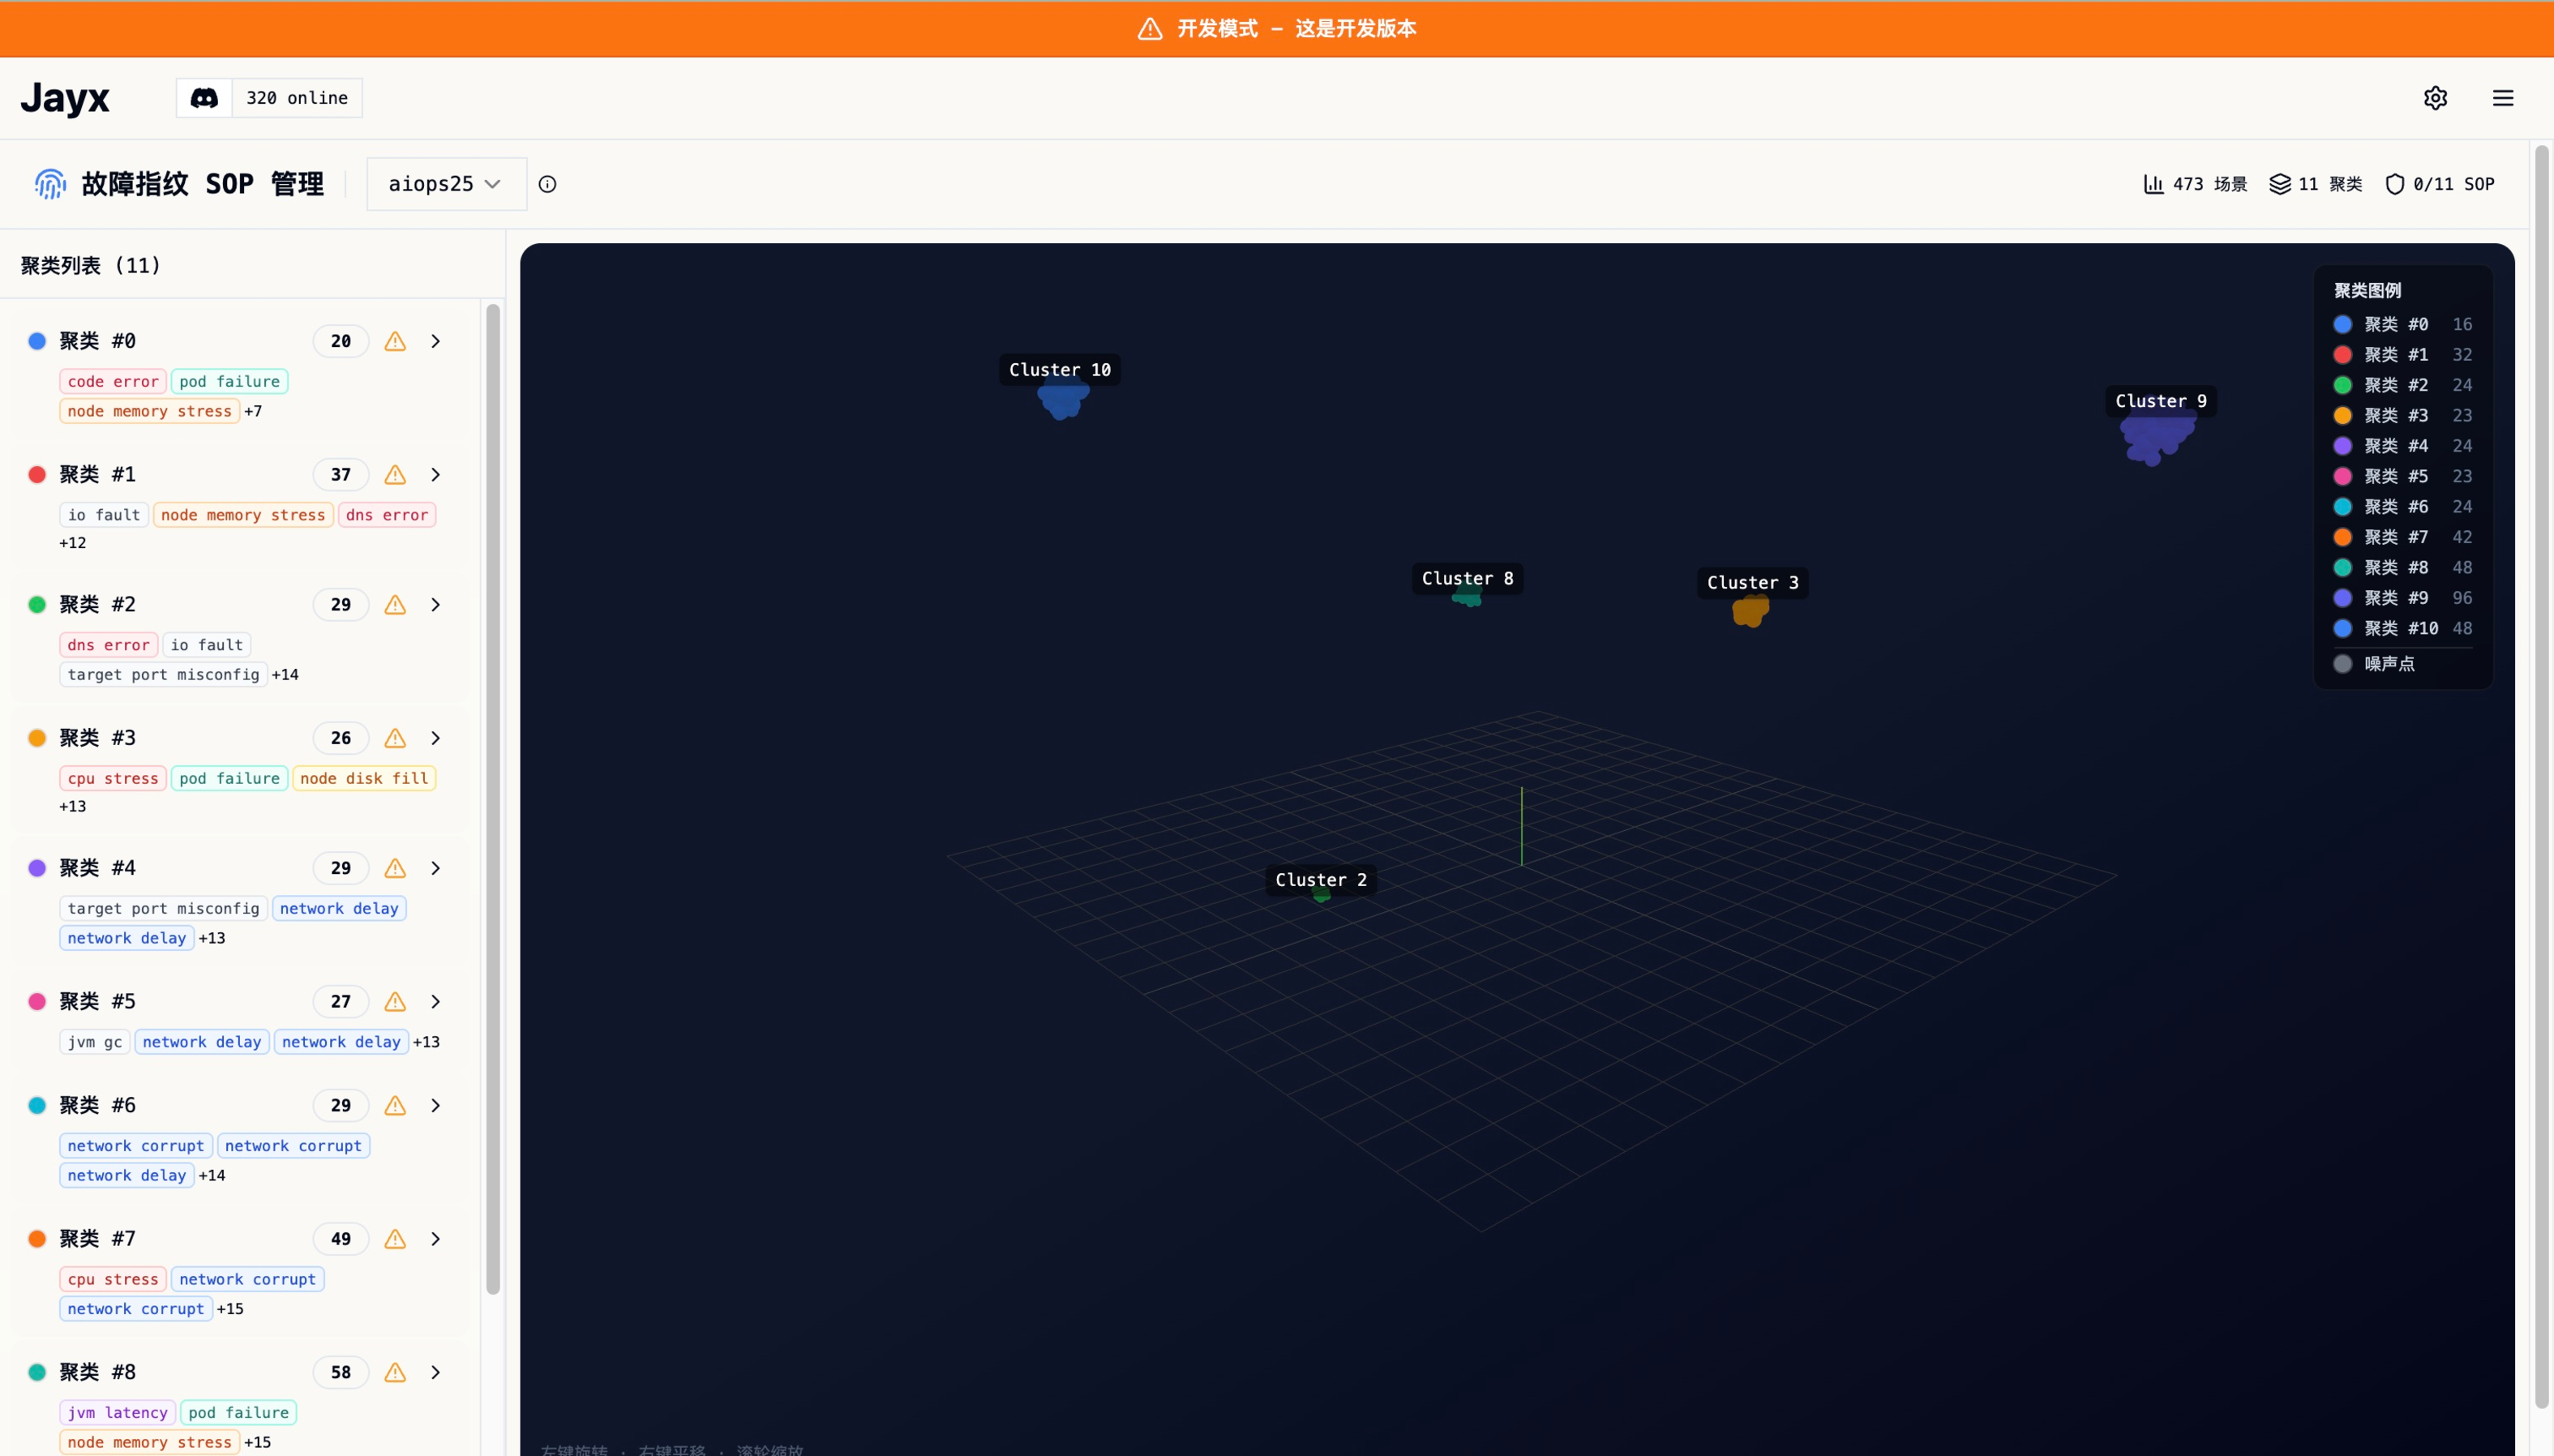
\includegraphics[width=0.96\textwidth]{Figures-Src/Chap4-System/user-interaction/fig3-fingerprint-3d.pdf}
    \bicaption{\enspace 三维嵌入空间中的故障指纹聚类分布}{\enspace Fault Fingerprint Clusters in a 3D Embedding Space}
    \label{fig:user_fingerprint_3d}
\end{figure}
\FloatBarrier

图中每个点对应一个故障实例，颜色表示其所属聚类。用户可以通过该界面定位特定聚类，查看其代表标签、样本规模和空间分布，并结合实例信息检查故障指纹库中的聚类结果。该界面主要用于故障指纹知识的展示与分析，为故障簇分布观察、聚类结果验证和相似故障关系理解提供辅助支持。

综上，诊断执行界面主要用于展示在线诊断过程及其对应的 SOP 路径状态，工作区界面主要用于组织案例级任务及其中间结果，故障指纹界面主要用于查看故障指纹库中的聚类结果与样本分布。三类界面分别服务于任务执行、任务管理与知识查看，共同构成了平台面向用户的主要交互界面。